\graphicspath{{chapters/08}}
\chapter{Quantum computing}
Not for the exam but perfect to read before going to bed!
\section{Qubits}
We can consider a quantum hamiltonian $\hat{H_0}$ that describes a two-level system. We can represent it with the same mathematical representation of spin even if it's not spin.
\[
\ket{0}=\begin{pmatrix}1\\0\end{pmatrix};\,
\ket{1}=\begin{pmatrix}0\\1\end{pmatrix}\,
\text{with}\,
\,\hat{H_0}=-h\hat{\tau_x},\,
\hat{\tau_x}=\begin{pmatrix}0&1\\1&0\end{pmatrix}
\text{Pauli matrix operator}
\]
\[
\hat{H_0}=-h\begin{pmatrix}0&1\\1&0\end{pmatrix}
\]
Questions, find:
\begin{itemize}
	\item$\ket{\hat{\Omega}}=\ket{\text{Ground state of }\hat{H_0}}$
	\item$\ket{\hat{\Sigma}}=\ket{\text{First excited state of }\hat{H_0}}$
\end{itemize}
To find the possible states of the hamiltonian first solve $\hat{H_0}\ket{\phi}=E\ket{\phi}$:
\[\det(H-\lambda \mathbb{1})=0\]
\[\det\begin{pmatrix}-\lambda&-h\\-h&-\lambda\end{pmatrix}=0\]
\[\lambda^2-h^2=0 \rightarrow \lambda=\pm h\]
$-h$ and $+h$ are the two possible energy eigenvalues and correspond to the ground state and first excited state, respectively.\\
Let's compute the \ul{ground state}: $E_\Omega=-h$
\[\ket{\Omega}=\begin{pmatrix}a\\b\end{pmatrix}\,\rightarrow\,
-h\begin{pmatrix}0&1\\1&0\end{pmatrix}\begin{pmatrix}a\\b\end{pmatrix}=-h\begin{pmatrix}a\\b\end{pmatrix}\]
This is a two-variables system and can be resolved as such:
\[
\begin{cases}-ha=-ha\\-hb=-hb\end{cases}\rightarrow a=0\, \text{and}\, b=1\, \text{or}\, a=1\, \text{and}\, b=0
\]
We can rewrite $\ket{\Omega}$ as
\[\ket{\Omega}=\frac{1}{\sqrt{2}}\ket{1}+\frac{1}{\sqrt{2}}\ket{0}\]
and since $\ket{1}=\begin{pmatrix}0\\1\end{pmatrix}$, I have to normalize the ket to get the $\begin{pmatrix}1\\1\end{pmatrix}$ that is the final result. Anyway, $\ket{\Omega}$ is a quantum superposition of states.\\
\ul{First excited state} $E_\Sigma=+h$
\[\ket{\Sigma}=\begin{pmatrix}a\\b\end{pmatrix}\,\rightarrow\,
-h\begin{pmatrix}0&1\\1&0\end{pmatrix}\begin{pmatrix}a\\b\end{pmatrix}=+h\begin{pmatrix}a\\b\end{pmatrix}\]
From this linear system we obtain the formulation for the first excited state.
\[\ket{\Sigma}=\frac{1}{\sqrt{2}}\ket{1}-\frac{1}{\sqrt{2}}\ket{0}\]
Each of these two quantum states, $\ket{\Omega}$ and $\ket{\Sigma}$, represent a \textbf{qubit} that is in a linear superposition of states.\\
\subsection{Adiabatic Quantum Computing}
Putting energy in the system chenges the probability of the particle of being still in a ground state. I may find the particle in an excited state. This doesn't happen if I switch the system in a slow manner (adiabatic system). I can never end up in an excited state $\rightarrow$ ADIABATIC THEOREM.\\
The transition is more likely to occur at the time when $\Delta E$ is at its lowest.\\
If $\hat{H_f}$ is complicated enough such as I can't know its ground state I can start from $\hat{H_0}$ ground state and let the system evoke in an adiabatic way to reach $\hat{H_f}$ ground state spontaneously and measure the final state many times.\\
I can obtain the final wavefunction by means of qubits. where qubits are two level-systems that can thus have two levels of energy. I know the two ground states. \\
\begin{figure}[htbp!]
	\centering
	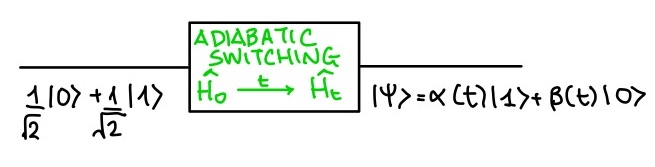
\includegraphics[scale=0.30]{img_10}
\end{figure}
I can compute the final solution by knowing the amount of values of $\alpha(t)$ and $\beta(t)$.\\
Time needed depends on the triviality of the problem, the larger number of qubits $(n)$, the larger number of states ($2^n$) and $\Delta E$, the most time, unless I have uncertainty. This depends on the function that "regulates" the $\Delta E$. The function corresponds to the \textit{clock} on classical computers that is how often registers are updated.\\

\section{Two qubits system}
Interacting quantum systems. Solve the Hamiltonian in the form:
\[
\hat{H}=\mathbf{J}_{12}\hat{\tau_1^z}\hat{\tau_2^z}+h(\hat{\tau_1^z}+\hat{\tau_2^z})
\]
This is a two-particles Hamiltonian that depends on the interaction of the two spins. If one of the two is down, $\hat{H}$ becomes negative and the energy is lowered. Hence I have a more favourable system. \\
I can obtain this with a magnet that can properly align spins in order to have an overall negative energy. Implicitally, the Hamiltonian should be:
\[
\hat{H}=\mathbf{J}_{12}\hat{\tau_1^z}\hat{\tau_2^z}+h(\hat{\tau_1^z}\hat{\mathbb{1}_z}+\hat{\mathbb{1}_z}\hat{\tau_2^z})
\]
When you use an operator on a particle, you multiply the other by the identity matrix.
\[
\hat{\tau_1^z}\otimes\hat{\tau_2^z}=\begin{pmatrix}1&0&0&0\\0&-1&0&0\\0&0&-1&0\\0&0&0&1\end{pmatrix}\,\,
\hat{\tau_1^z}\otimes\hat{\mathbb{1}_z}=\begin{pmatrix}1&0&0&0\\0&1&0&0\\0&0&-1&0\\0&0&0&-1\end{pmatrix}\,\,
\hat{\mathbb{1}^z}\otimes\hat{\tau_2^z}=\begin{pmatrix}1&0&0&0\\0&-1&0&0\\0&0&1&0\\0&0&0&-1\end{pmatrix}
\]
The Hamiltonian then becomes
\[
\hat{H}=\mathbf{J}_{12}\begin{pmatrix}1&0&0&0\\0&-1&0&0\\0&0&-1&0\\0&0&0&1\end{pmatrix}+h\begin{pmatrix}2&0&0&0\\0&0&0&0\\0&0&0&0\\0&0&0&-2\end{pmatrix}=\begin{pmatrix}\mathbf{J}_{12}+2h&0&0&0\\0&-\mathbf{J}_{12}&0&0\\0&0&-\mathbf{J}_{12}&0\\0&0&0&-2h+\mathbf{J}_{12}\end{pmatrix}
\]
Each of the eigenvalues of the matrix can represent an eigenvector.\\
\newline
Suppose we have a function defined as a quadratic function of binary variables:
\[
T=\sum_{i,j=1}^N O_{ij}x_ix_j+\sum_i^N U_ix_i \text{ with } x_i\in \{0,1\} \text{ and } O_{ij},U_i\in \mathbb{R}
\]
The problem is finding the configuration of binary variables that minimises $T$. This is a discrete optimization problem that is called \textbf{Quadratic Unconstrained Binary Optimization (QUBO)} problem.\\
We can reduce the two-particle problem to a QUBO problem.\\
By definition $\hat{\tau_i^z}=2x_i-1$\\
When \[\begin{matrix}x_i=0&\hat{\tau_i^z}=-1\\x_i=1&\hat{\tau_i^z}=+1 \end{matrix}\]
We can write the function $T$ as
\[
T=\sum_{i,j=1}^N \mathbf{J_{ij}}\tau_i^z\tau_j^z+\sum_i^N h_i\tau_i^z
\]
that is similar to the original Hamiltonian. I have a total number of combination of $2^N$. Values of $T$ are encoded in the Hamiltonian. Results of finding the minimum of $T$ and $\hat{H}$ are the same because the minimum value of the ground state corresponds to the ground eigenstate. \\
The qubits corresponding to the ground eigenstate (eigenvectors) can be obtained from classical $T$ but not as a superposition.\\
I can create entangled states by imposing a different spin direction on the particles.
\[
\hat{H}=\mathbf{J}_{12}\hat{\tau_1^z}\hat{\tau_2^z}+h(\hat{\tau_1^x}\hat{\mathbb{1}_x}+\hat{\mathbb{1}_x}\hat{\tau_2^x})
\]
\[\hat{\tau_1^x}\otimes\hat{\mathbb{1}_x}=\begin{pmatrix}0&0&1&0\\0&0&0&1\\1&0&0&0\\0&1&0&0\end{pmatrix}\,\,
\hat{\mathbb{1}^x}\otimes\hat{\tau_2^x}=\begin{pmatrix}0&1&0&0\\1&0&0&0\\0&0&0&1\\0&0&1&0\end{pmatrix}\,\,
\hat{H}=\begin{pmatrix}\mathbf{J}_{12}&h&h&0\\h&-\mathbf{J}_{12}&0&h\\h&0&-\mathbf{J}_{12}&h\\0&h&h&\mathbf{J}_{12}\end{pmatrix}\]
The ground state is a vector correspondant to
\[
\begin{pmatrix}1\\0\\-\frac{\sqrt{4h^2+\mathbf{J}^2}+\mathbf{J}}{2h}\\1 \end{pmatrix}=\ket{0\,0}-\frac{\sqrt{4h^2+\mathbf{J}^2}+\mathbf{J}}{2h}\ket{1\,0}+\ket{1\,1}
\]
Where $c=\frac{\sqrt{4h^2+\mathbf{J}^2}+\mathbf{J}}{2h}$\\
Normalization factor:
\[
\frac{(1^2+c^2+1^2)}{N}=1 \rightarrow N=2+c^2
\]
\[
G.S.=\frac{1}{\sqrt{2+c^2}}(\ket{0\,0}-c\,\ket{1\,0}+\ket{1\,1})
\]
Let's fix $c=1$ so the ground state becomes:
\[
G.S.= \frac{1}{\sqrt{3}}(\ket{0\,0}-\ket{1\,0}+\ket{1\,1})
\]
Let's calculate the probability for $q_2=1$. $q_2$ can appear in two different states:
\[P_{1 1}=\frac{1}{3}(\braket{1\,1\,|\,0\,0}-\braket{1\,1\,|\,1\,0}+\braket{1\,1\,|\,1\,1})^2=\bigg(\frac{1}{\sqrt{3}}\bigg)^2=\frac{1}{3}\]
\[P_{0 1}=\frac{1}{3}(\braket{0\,1\,|\,0\,0}-\braket{0\,1\,|\,1\,0}+\braket{0\,1\,|\,1\,1})^2=0\]
This latter state never appears.\\
The state is overall entangled because if $q_1=0$ the wave function collapses into $q_2=0$. If $q_1=1$, $q_2$ doesn't collapse because it can be either $q_2=0$ or $q_2=1$ with 50\% probability. $q_2$ is in a linear superposition of states if $q_1=1$.\\

\section{Quantum circuits}
Quantum circuits are models for \textbf{quantum computation},
\marginpar{\textit{This divulgative fragment is from Wikipedia, Quantum Inspire, Qiskit}}
where a computation is a sequence of quantum gates, measurements, and initialization of qubits to known values et cetera. Circuits are written such as horizontal axis is time, they are read from left to right. Horizontal lines represent qubits, doubled lines are classical bits. The items that connect the elements represents the operations performed on qubits.\\
Most\textbf{ elementary logic gates} (= model of computation or physical electronic device that implements a boolean function on one or more binary inputs) are \textbf{irreversible}, this means that if I have a \textit{AND gate} applied on two bits, I cannot recover these two bits from the result.\\
Quantum computers can achieve \textbf{universality}, i.e., the complete conversion of an input of an arbitrary set of items into a corresponding output. Usually in quantum computation the output is a rotation of the input, I can express all the operations used to perform such rotation $f(x)$ on input $x$ as a single unitary matrix, for example
\[
U=\sum_j\ket{f(x)}\bra{x}
\]
The ability to implement any unitary matrix would mean the achievement of universality in the sense of standard digital computers. A strictly physical example would be the simulation of the dynamics of a system, the time evolution is the unitary, the Hamiltonian is the associated hermitian matrix. Achieving any unitary would therefore correspond to simulating any time evolution, and engineering the effects of any Hamiltonian.\\

\textbf{Quantum logic gates} are \underline{reversible unitary transformations} on at least one qubit. We must first define a qubit (the quantized version of classical \textit{n}-bit space $\{0,1\}^n$) is the Hilbert space $H_{QB(n)}=L^2(\{0,1\}^2)$, that can be interpreted as a linear combinations/superpositions of classical bit strings. $H_{QB(n)}$ is a vector space over the complex numbers of dimension $2^n$, the elements of this vector space are the possible state of \textit{n}-qubits quantum registers. Quantum logic gates require a reversible function called unitary mapping (linear transformation of a complex inner product space that preserves the Hermitian inner product).\\
There are three main types of quantum circuits:
\begin{itemize}
\item \textbf{Phase gate (S gate)}: single-qubit operation defined by the matrix
$S=\begin{pmatrix}1&0\\0&i \end{pmatrix}$, it represents a 90-degree rotation around the z-axis.
\item \textbf{Hadamard gate}: single-qubit operation that maps the basis state $\ket{0}$ to $\frac{\ket{0}+\ket{1}}{\sqrt{2}}$ and $\ket{1}$ to $\frac{\ket{0}-\ket{1}}{\sqrt{2}}$ thus creates a superposition of the two basis states. It can be represented by the matrix $H=\frac{1}{\sqrt{2}}\begin{pmatrix} 1&1\\1&-1\end{pmatrix}$. It represents a 90$^{\circ}$ rotation around the Y-axis followed by a 180$^{\circ}$ rotation around the X-axis.
\item \textbf{CNOT gate}: two-qubit operation. The \underline{first qubit} is the CONTROL QUBIT, the \underline{second qubit} is the TARGET QUBIT. This gate leaves the control qubit unchanged and performs a Pauli-X gate on the target qubit if control is $\ket{1}$. If control is $\ket{0}$ the target qubit is unchanged. The CNOT gate is represented by the matrix $C_{NOT} = \begin{pmatrix}1&0&0&0\\0&1&0&0\\0&0&0&1\\0&0&1&0 \end{pmatrix}$
\end{itemize}
\begin{figure}[htbp!]
	\centering
	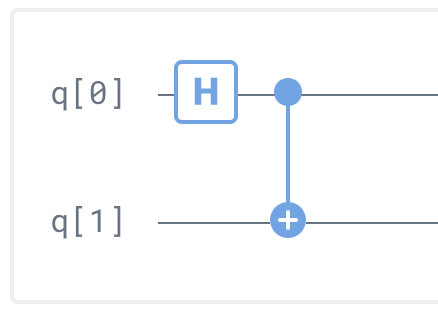
\includegraphics[scale=0.30]{img_11}
\end{figure}
The figure represents the execution of Hadamard gate on qubit 0 to create a superposition state and then the execution of CNOT gate to create an entangled state of the two qubits.\\

\textit{Exercise 1 - Prove that Hadamard gate is the reverse of itself}\\
\[H=\frac{1}{\sqrt{2}}\begin{pmatrix}1&1\\1&-1\end{pmatrix}\,\,\ket{0}=\begin{pmatrix}1\\0\end{pmatrix}\,\,\ket{1}=\begin{pmatrix}0\\1\end{pmatrix}\]
\[H\,\ket{0}=\frac{1}{\sqrt{2}}\begin{pmatrix}1&1\\1&-1\end{pmatrix}\begin{pmatrix}1\\0\end{pmatrix}=\frac{1}{\sqrt{2}}\begin{pmatrix}1+0\\1+0\end{pmatrix}=\begin{pmatrix}1/\sqrt{2}\\1/\sqrt{2}\end{pmatrix}\]
\[
H\,(H\,\ket{0})=\frac{1}{\sqrt{2}}\begin{pmatrix}1&1\\1&-1\end{pmatrix}\begin{pmatrix}1/\sqrt{2}\\1/\sqrt{2}\end{pmatrix}=\frac{1}{\sqrt{2}}\begin{pmatrix}1/\sqrt{2}+1/\sqrt{2}\\1/\sqrt{2}-1/\sqrt{2}\end{pmatrix}=\frac{1}{\sqrt{2}}\begin{pmatrix}2/\sqrt{2}\\0\end{pmatrix}=\begin{pmatrix}1\\0\end{pmatrix} \text{Q.E.D.}\]
It's pointless to put two Hadamard gates in a row from a mathematical point of view. From a physical point of view it means that I am restoring the cat in an aline/dear definite state that is technically not possible.\\
\newline

\textit{Exercise 2 - Example of a $HC_{NOT}$ quantum circuit}\\\newline
Application of the two gates on different entangled states of qubits $\ket{0}$ and $\ket{1}$.
\[
C_{NOT}(H\,\ket{0\,0})=C_{NOT}(H\,\ket{0}\otimes\ket{0})=C_{NOT}\bigg(\frac{1}{\sqrt{2}}\begin{pmatrix}1&1\\1&-1\end{pmatrix}\begin{pmatrix}1\\0\end{pmatrix}\otimes\begin{pmatrix}1\\0\end{pmatrix}\bigg)=C_{NOT}\bigg(\frac{1}{\sqrt{2}}\begin{pmatrix}1\\1\end{pmatrix}\otimes\begin{pmatrix}1\\0\end{pmatrix}\bigg)=
\]
\[
=C_{NOT}\frac{1}{\sqrt{2}}\begin{pmatrix}1\\0\\\mathcolorbox{yellow}{1}\\\mathcolorbox{yellow}{0}\end{pmatrix}=\frac{1}{\sqrt{2}}\begin{pmatrix}1&0&0&0\\0&1&0&0\\0&0&0&1\\0&0&1&0\end{pmatrix}\begin{pmatrix}1\\0\\1\\0\end{pmatrix}=\frac{1}{\sqrt{2}}\begin{pmatrix}1+0+0+0\\0+0+0+0\\0+0+0+0\\0+0+1+0\end{pmatrix}=\frac{1}{\sqrt{2}}\begin{pmatrix}1\\0\\\mathcolorbox{yellow}{0}\\\mathcolorbox{yellow}{1}\end{pmatrix}=\frac{\ket{0\,0}+\ket{1\,1}}{\sqrt{2}}=\ket{\phi^+}
\]
As foreseen in the theory, the second qubit changes when the $C_{NOT}$ gate is applied. The result is an entangled state of the two qubits called \textbf{BELL STATE}. All Bell states resulting from the combinations are orthogonal to each other.
\[\frac{\ket{0\,0}-\ket{1\,1}}{\sqrt{2}}=\ket{\phi^-}\,\,\frac{\ket{0\,1}+\ket{1\,0}}{\sqrt{2}}=\ket{\psi^+}\,\,\frac{\ket{0\,1}-\ket{1\,0}}{\sqrt{2}}=\ket{\psi^-}\]
\[\braket{\psi^+\,|\,\psi^-}=0\]
\section{The Elitzur-Vaidman bomb tester}
The Elitzur-Vaidman bomb tester is a quantum mechanics thought experiment that uses interaction-free mechanism to verify that a bomb is functional without having to detonate it. \\
This experiment uses two characteristics of elementary particles: \textbf{nonlocality} and \textbf{wave-particle duality}. The fundamentals of this experiment can be explained with an example: if we have two closed boxes and we know that in one of the two there is an object, by opening one and finding it empty, we know that the object is in the other one without opening it.\\
The particle, during the experiment, is in a superposition of states/locations, it can be anywhere in any moment. The particle's wave can be collapsed by observing it to obtain its local information. I can obtain information about previous positions of the particle before the collapse and even in cases where the particle was never in those positions.\\
\begin{figure}[htbp!]
	\centering
	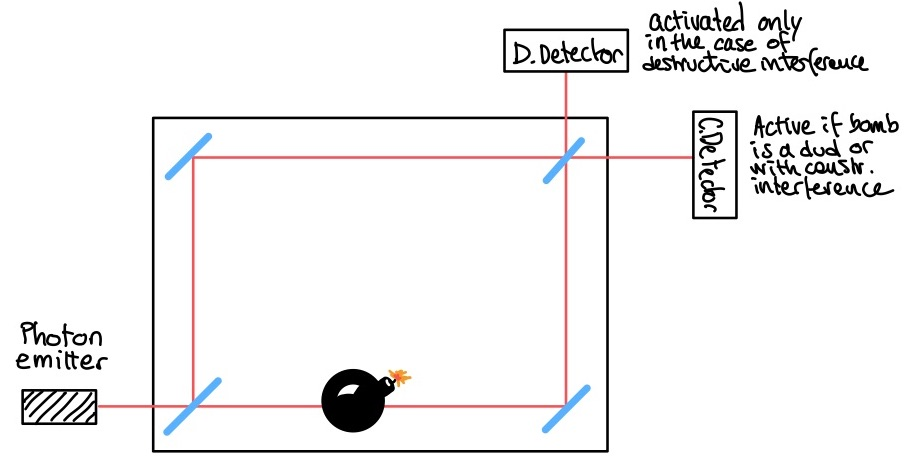
\includegraphics[scale=0.30]{img_12}
\end{figure}

\ul{Bomb not inserted}:\\
When the photon is emitted and it reaches the first beam splitter, a superposition of states is created, the photon can either go to the upper path or to the lower path with a 50\% probability each. The photon encounters two mirrors that reflect the beam and the two meet at a second beam splitter that directs the beam to two detectors with the same probability:
\begin{itemize}
	\item C Detector: reached by the transmitted beam. Activated by the constructive interference of the two photons behaving as waves.
	\item D Detector: reached by the reflected beam. Never activated in normal conditions (destructive interference happens hence no signal)
	\end{itemize}
When the bomb is dud, C detector has a 100\% probability of detecting a signal, the superposition of states created by the first beam splitter create a constructive interference that is detected by C (I have destructive interference in D so nothing is detected).\\
With this being said, three things may happen when \ul{the bomb is inserted and LIVE}:
\begin{itemize}
	\item 50\% THE BOMB EXPLODES: The photon took the lower path and activated the bomb. The activation of the bomb can be considered as a collapse of the wave function, the photon never arrives at the detector and no signal is present.
	\item 25\% PHOTON DETECTED AT C: The photon took the upper way and was transmitted by the second beam splitter.
	\item 25\% PHOTON DETECTED AT D: The photon took the upper way and was reflected by the second beam splitter. The presence of a signal at detector D is the only way to know whether the bomb is live without its explosion.
	\end{itemize}
